\documentclass[a4paper]{article}
\usepackage[utf8]{inputenc}
\usepackage{amsmath}
\usepackage{amssymb}
\usepackage{caption}
\usepackage{mathtools}
\usepackage{amsfonts}
\usepackage{lastpage}
\usepackage{tikz}
\usepackage{float}
\usepackage{textcomp}
\usetikzlibrary{patterns}
\usepackage{pdfpages}
\usepackage{gauss}
\usepackage{fancyvrb}
\usepackage[table]{colortbl}
\usepackage{fancyhdr}
\usepackage{graphicx}
\usepackage[margin=2.5 cm]{geometry}

\definecolor{listinggray}{gray}{0.9}
\usepackage{listings}
\lstset{
	language=,
	literate=
		{æ}{{\ae}}1
		{ø}{{\o}}1
		{å}{{\aa}}1
		{Æ}{{\AE}}1
		{Ø}{{\O}}1
		{Å}{{\AA}}1,
	backgroundcolor=\color{listinggray},
	tabsize=3,
	rulecolor=,
	basicstyle=\scriptsize,
	upquote=true,
	aboveskip={0.2\baselineskip},
	columns=fixed,
	showstringspaces=false,
	extendedchars=true,
	breaklines=true,
	prebreak =\raisebox{0ex}[0ex][0ex]{\ensuremath{\hookleftarrow}},
	frame=single,
	showtabs=false,
	showspaces=false,
	showlines=true,
	showstringspaces=false,
	identifierstyle=\ttfamily,
	keywordstyle=\color[rgb]{0,0,1},
	commentstyle=\color[rgb]{0.133,0.545,0.133},
	stringstyle=\color[rgb]{0.627,0.126,0.941},
  moredelim=**[is][\color{blue}]{@}{@},
}

\lstdefinestyle{base}{
  emptylines=1,
  breaklines=true,
  basicstyle=\ttfamily\color{black},
}

\pagestyle{fancy}
\def\checkmark{\tikz\fill[scale=0.4](0,.35) -- (.25,0) -- (1,.7) -- (.25,.15) -- cycle;}
\newcommand*\circled[1]{\tikz[baseline=(char.base)]{
            \node[shape=circle,draw,inner sep=2pt] (char) {#1};}}
\newcommand*\squared[1]{%
  \tikz[baseline=(R.base)]\node[draw,rectangle,inner sep=0.5pt](R) {#1};\!}
\newcommand{\comment}[1]{%
  \text{\phantom{(#1)}} \tag{#1}}
\newcommand{\pd}[2]{%
  \frac{\partial^{#2}}{\partial #1^{#2}}}
\def\el{[\![}
\def\er{]\!]}
\def\dpip{|\!|}
\def\MeanN{\frac{1}{N}\sum^N_{n=1}}
\cfoot{Page \thepage\ of \pageref{LastPage}}
\DeclareGraphicsExtensions{.pdf,.png,.jpg}
\author{Nikolaj Dybdahl Rathcke (rfq695) \\
        Victor Petren Bach $\Re$øvhul Hansen (grn762) \\
        Tobias Hallundbæk Petersen (xtv657) }
\title{Signal and Image Processing \\ Assignment 4}
\lhead{SIP}
\rhead{Assignment 4}

\begin{document}
\maketitle
\section{Question 1}
The code for this question is seen below:
\lstinputlisting[language=Matlab]{src/q1.m}
We want to show that a convolution of a gaussian with itself is also gaussian by calculating images from its scale-space. The filter \texttt{A} is a gaussian kernel with sigma equal to the parameter $s$, which is $3$. To calculate an image from its scale space, we use the handed out \texttt{scale} with parameter $t=4$, called tau. The other image is calculated directly using $\sigma=\sqrt{s^2+t^2}$. The output from running the file is two images, which are shown in Figure \ref{q1_1}.
\begin{figure}[H]
  \centering
  \captionsetup{justification=centering}
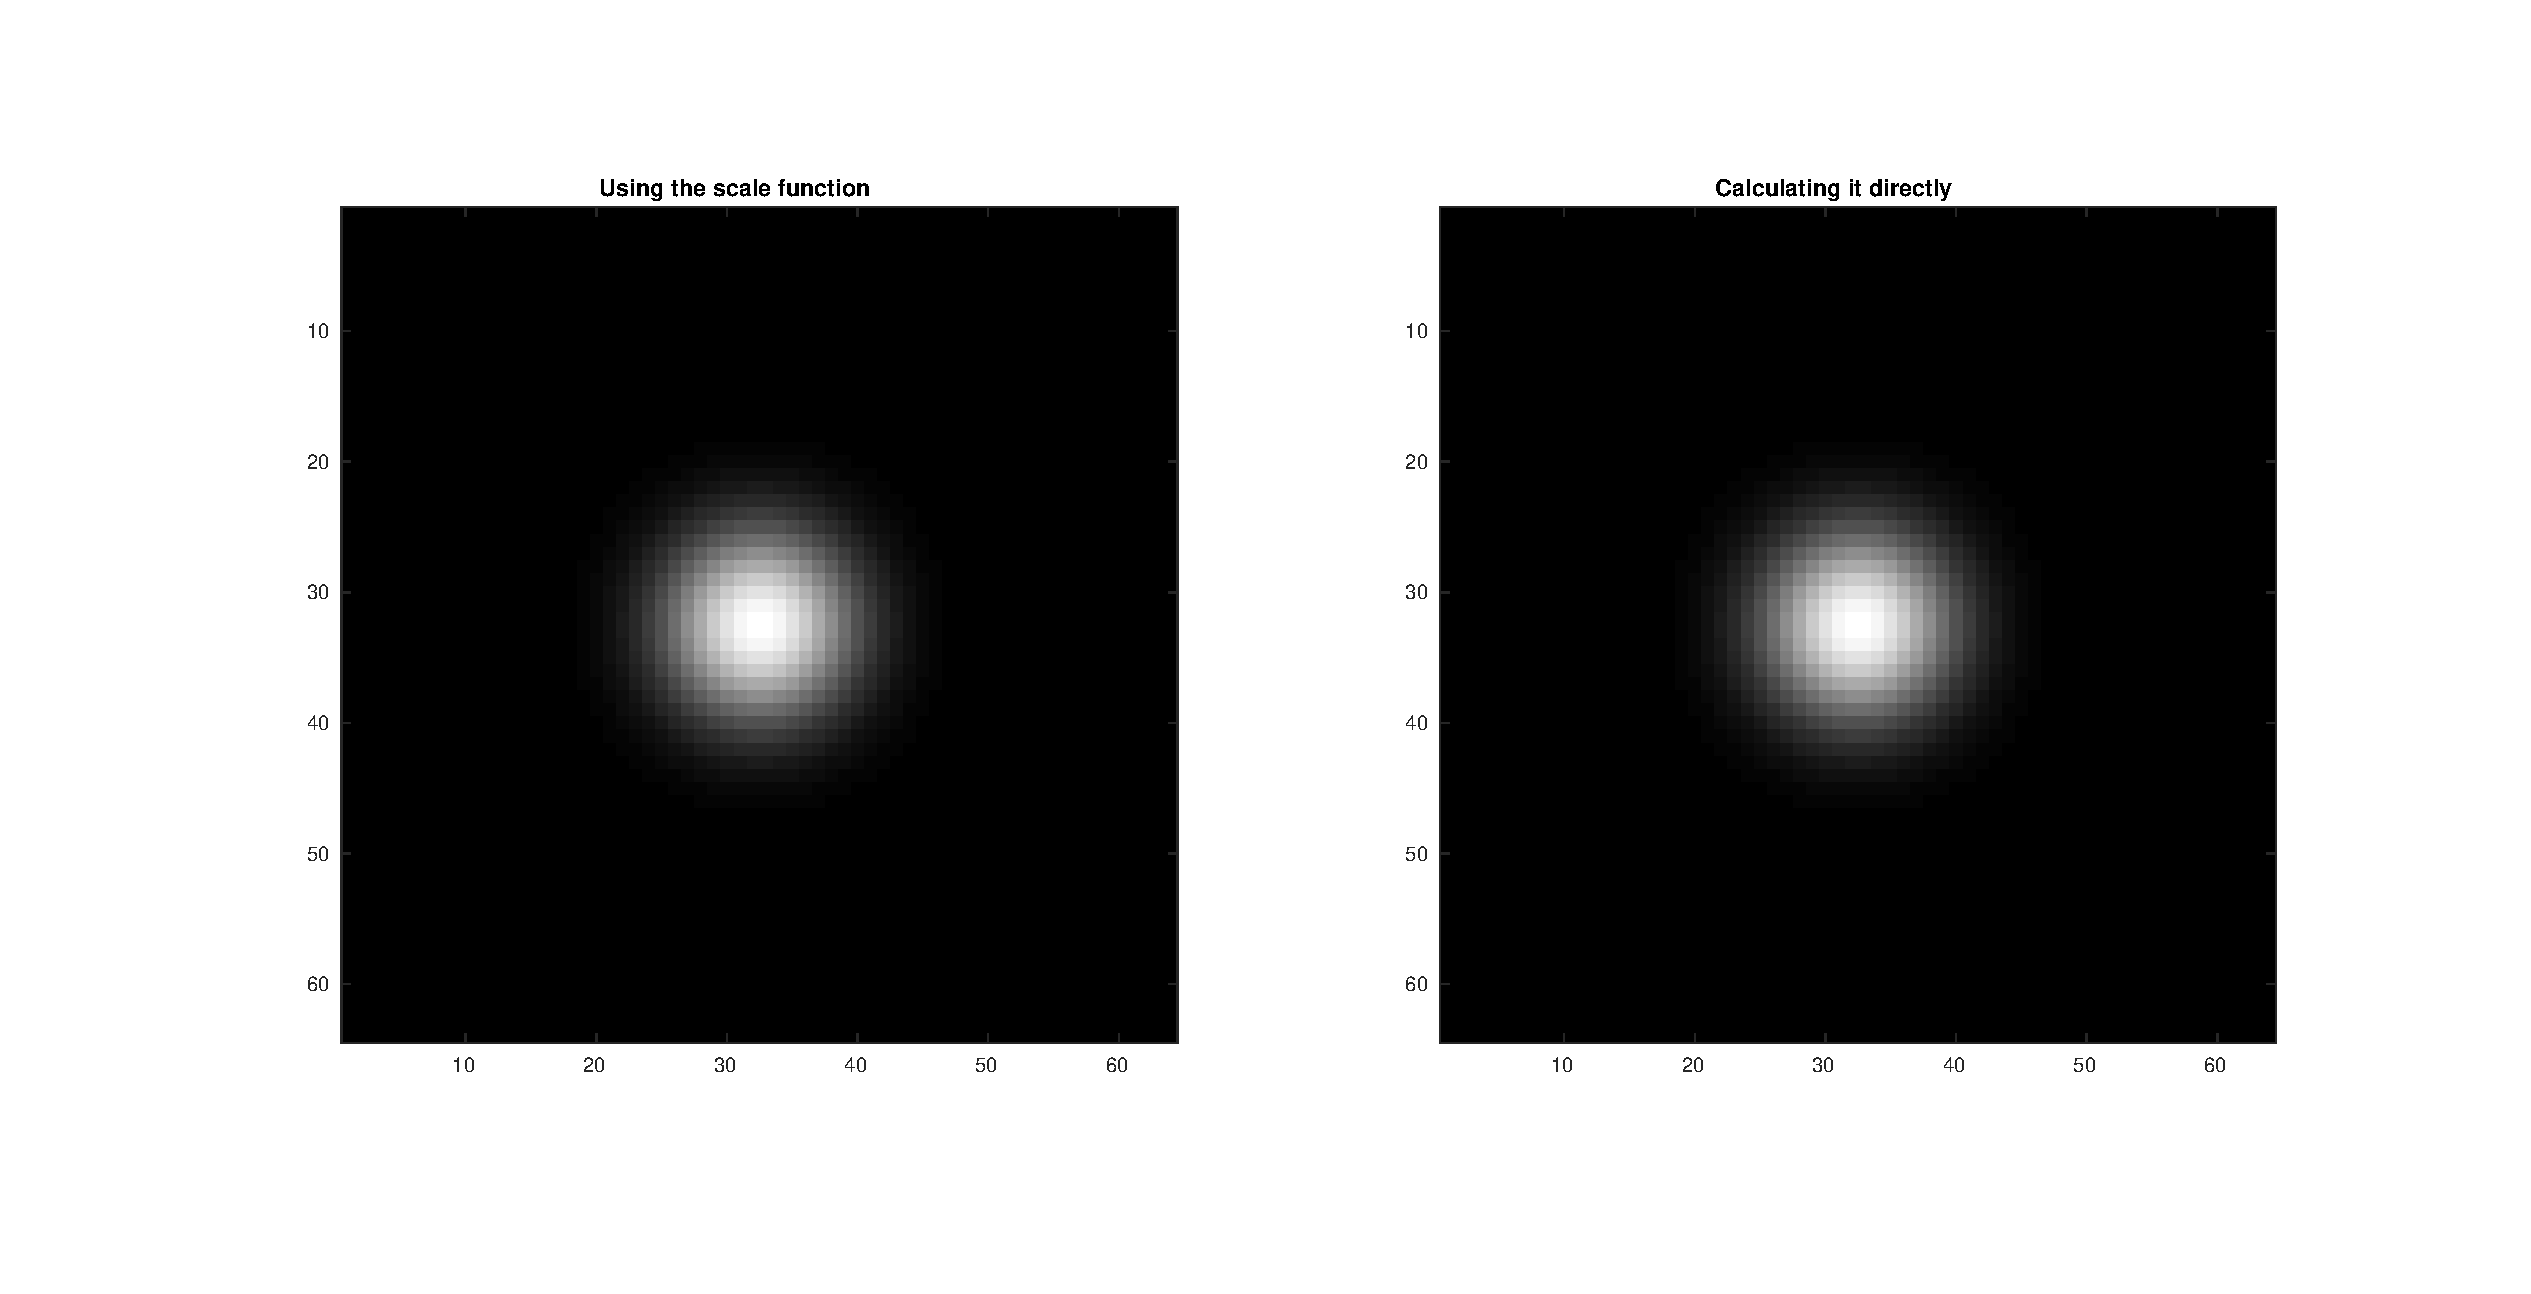
\includegraphics[width=\textwidth]{q1_1.eps}
  \caption{Figure showing the resulting images from calculating a convolution of a gaussian with itself by its scale space and directly.}
  \label{q1_1}
\end{figure}
Even though the images seem to be identical, this is not the case. However, the error is very small. The mean squared error between the two approaches is $2.3440\cdot10^{-25}$, so the images are very similar.

\section{Question 2}
\subsection{(a)}
We want to calculate the analytical expression for $H(x,y,\tau)$ for $\gamma = 1$.
\begin{align*}
  H(x,y,\tau) &= I_{xx}(x,y,\tau) + I_{yy}(x,y,\tau)\\
  &= \tau^2 \left( \pd{x}{2} I(x,y,\tau) \pd{y}{2} I(x,y,\tau) \right) \comment{Using (5)}\\
  &= \tau^2 \left( \pd{x}{2} G(x,y,\sqrt{\tau^2 + \sigma^2}) + \pd{y}{2} G(x,y,\sqrt{\tau^2 + \sigma^2})\right) \comment{Using (2), (3) and (4)}\\
  &= \tau^2 \left( \pd{x}{2} \left(\frac{1}{2\pi(\tau^2 + \sigma^2)}e^{-\frac{x^2 + y^2}{2(\tau^2 + \sigma^2)}}\right) + \pd{y}{2} \left(\frac{1}{2\pi(\tau^2 + \sigma^2)}e^{-\frac{x^2 + y^2}{2(\tau^2 + \sigma^2)}}\right) \right) \comment{Using (1)}\\
  &= \tau^2 \left(\frac{2x^2e^{- \frac{x^2+y^2}{2\sigma^2 +2\tau^2}}}{(2\sigma^2 + 2\tau^2)^2\pi(\sigma^2 + \tau^2)}- \frac{e^{- \frac{x^2+y^2}{2\sigma^2 +2\tau^2}}}{(2\sigma^2 + 2\tau^2)\pi(\sigma^2 + \tau^2)}\right) + \\
  &\phantom{=} \tau^2\left(\frac{2y^2e^{- \frac{x^2+y^2}{2\sigma^2 +2\tau^2}}}{(2\sigma^2 + 2\tau^2)^2\pi(\sigma^2 + \tau^2)}- \frac{e^{- \frac{x^2+y^2}{2\sigma^2 +2\tau^2}}}{(2\sigma^2 + 2\tau^2)\pi(\sigma^2 + \tau^2)}\right) \comment{Deriving the expression twice}\\
  &= - \frac{t^2 e^{-\frac{x^2 + y^2}{2\sigma^2 + 2\tau^2}}(2\sigma^2 + 2 \tau^2 - x^2 - y^2)}{2(\sigma^2 + \tau^2)^3 \pi} \comment{Simplified}
\end{align*}
Which is the analytical expression for $H(x,y,\tau)$.

\section*{Question 3}
\subsection*{a}
When having a soft edge defnied as following:
$$
  J(x,y)=\int^{x}_{-\infty} G(x',0,\sigma)dx'
$$
where its scale-space is defined as following:
$$
  J(x,y,\tau)=J(x,y)**G(x,y,\tau)
$$
Finding the $x$ and $y$ components of this is done as following. $J_x$ is found by taking the derivative of $J(x,y,\tau)$ w.r.t. $x$. As $J(x,y)$ is expressed as an integral, taking the derivative cancels it out, leaving the body of the integral:
\begin{align*}
  J_x &= \frac{\partial}{\partial x}(J(x,y) ** G(x,y,\tau)) \\
      &= \frac{\partial}{\partial x} (J(x,y)) ** G(x,y,\tau) \\
      &= G(x,0,\sigma) ** G(x,y,\tau)
\end{align*}
We can apply the same procedure for $J_y$, but as the y-component of the integral body is $0$, $J_y$ will be zero aswell:
\begin{align*}
  J_y &= \frac{\partial}{\partial y}(J(x,y) ** G(x,y,\tau)) \\
      &= 0
\end{align*}
we can therefore disregard $J_y$. The Gaussian kernel, $G(x,y,\tau)$, can be expreseed analytically by using equation (1):
$$
  G(x,y,\tau) = \frac{1}{2\pi \tau^2} e^{-\frac{x^2+y^2}{2\tau^2} }
$$
which now can be expressed in terms of the one-dimensional Gaussian kernel:
\begin{align*}
  G(x,y,\tau) &= \frac{1}{2\pi \tau^2} e^{-\frac{x^2+y^2}{2\tau^2} } \\
              &= \frac{1}{2\pi \tau^2} e^{-\frac{x^2}{2\tau^2} } e^{-\frac{y^2}{2\tau^2} }\\
              &= \frac{1}{\sqrt{2\pi \tau^2}} e^{-\frac{x^2}{2\tau^2} } \frac{1}{\sqrt{2\pi \tau^2}} e^{-\frac{y^2}{2\tau^2} }\\
              &= G(x,\tau)G(y,\tau)
\end{align*}
Now we can write $J_x$ where the integration only is done over one part of the expression
$$
J_x = \int_{-\infty}^{\infty}\int_{-\infty}^{\infty} G(x', 0,\tau) G(x-x',\tau) \:dx' \: G(y-y')\: dy'
$$
In order to simpify this expression, the following two observations can be used. \\
First of all, it can be seen that the integral of the $y$-component multiplied by any constant $k$,  will result in $k$, which removed the integral over this $y$-component:
$$
  \int^{\infty}_{-\infty} k G(y-y',\tau)\:dy' = k
$$
And secondly, we can use a modification of equation (2) for one dimension only, and the convolution can be expressed as:
$$
  G(x',0,\sigma)**G(x-x',\tau) = \hat{G}(x,\sqrt{\sigma^2 + \tau^2})
$$
which means we now can express $J_x$ as
$$
  J_x = \hat{G}(x,\sqrt{\sigma^2 +\tau^2})
$$
Here, $\hat{G}$ is the normalized expression for $G$, found the following way:
\begin{align*}
  G(x,0,\sigma) &= \frac{1}{2\pi\sigma^2}e^{-\frac{x^2}{2\sigma^2} } \\
                &= \frac{1}{\sqrt{2\pi\sigma^2}} (G(x,\sigma))\\
                &= \hat{G}(x,\sqrt{\sigma^2, \tau^2})
\end{align*}
Now that we have found $J_x$, the scale normalized derivative $J_x'$ must be found, which is done by using $\gamma = \frac{1}{2} $ $i=1$ and $j=0$ in equation (5):
$$
J_x' = \sqrt{\tau}J_x
$$
We can use this in equation (9) and get the desired analytical expression:
\begin{align*}
  |\!| \nabla I |\!|^2 &= J_x^2 + J_y^2\\
                       &= \tau (J_x^2 + J_y^2)\\
                       &= \tau \left( \frac{1}{\sqrt{ 2\pi\sigma^2}}G(x,\sqrt{\sigma^2 + \tau^2})  \right)\\
                       &= \frac{\tau}{\sqrt{2\pi\sigma^2}} \frac{1}{2\pi(\sigma^2 + \tau^2)} e^{- \frac{x^2}{2(\sigma^2 + \tau^2)} } \comment{last factor subst from eq (1)}
\end{align*}
\subsection*{b)}
We can find the scale for which the point in $(0,0)$ is maximal, by taking the derivative of the analytical expression found previously (with $x=0$):
$$
\frac{\tau}{\sqrt{2\pi\sigma^2}} \frac{1}{2\pi(\sigma^2 + \tau^2)} e^{- \frac{x^2}{2(\sigma^2 + \tau^2)} } = \frac{\tau}{\sqrt{2\pi\sigma^2}} \frac{1}{2\pi(\sigma^2 + \tau^2)}
$$
When taking the derivative of this expression w.r.t. $\tau$, we get the following:
$$
  \frac{\partial}{\partial \tau} \frac{\tau}{\sqrt{2\pi\sigma^2}} \frac{1}{2\pi(\sigma^2 + \tau^2)} = \frac{1}{4} \frac{\sqrt{2}}{\sqrt{\pi\sigma^2} \pi(\sigma^2 + \tau^2)}
$$
\subsection*{c)}
\subsection*{d)}

\section{Question 4}
The function \texttt{LSI} takes three parameters: An image, a kernel and a type of noise. It then convolves the image with the kernel and adds the given noise. Then function uses the default for any optional parameters. The function is seen below:
\lstinputlisting[language=Matlab]{src/LSI.m}
Running the function on the image \texttt{lena.tif} with a gaussian kernel and added gaussian noise produces the right image in Figure \ref{q4_1}. The gaussian kernel uses a $5$ by $5$ window and has $\sigma=1$.
\begin{figure}[H]
  \centering
  \captionsetup{justification=centering}
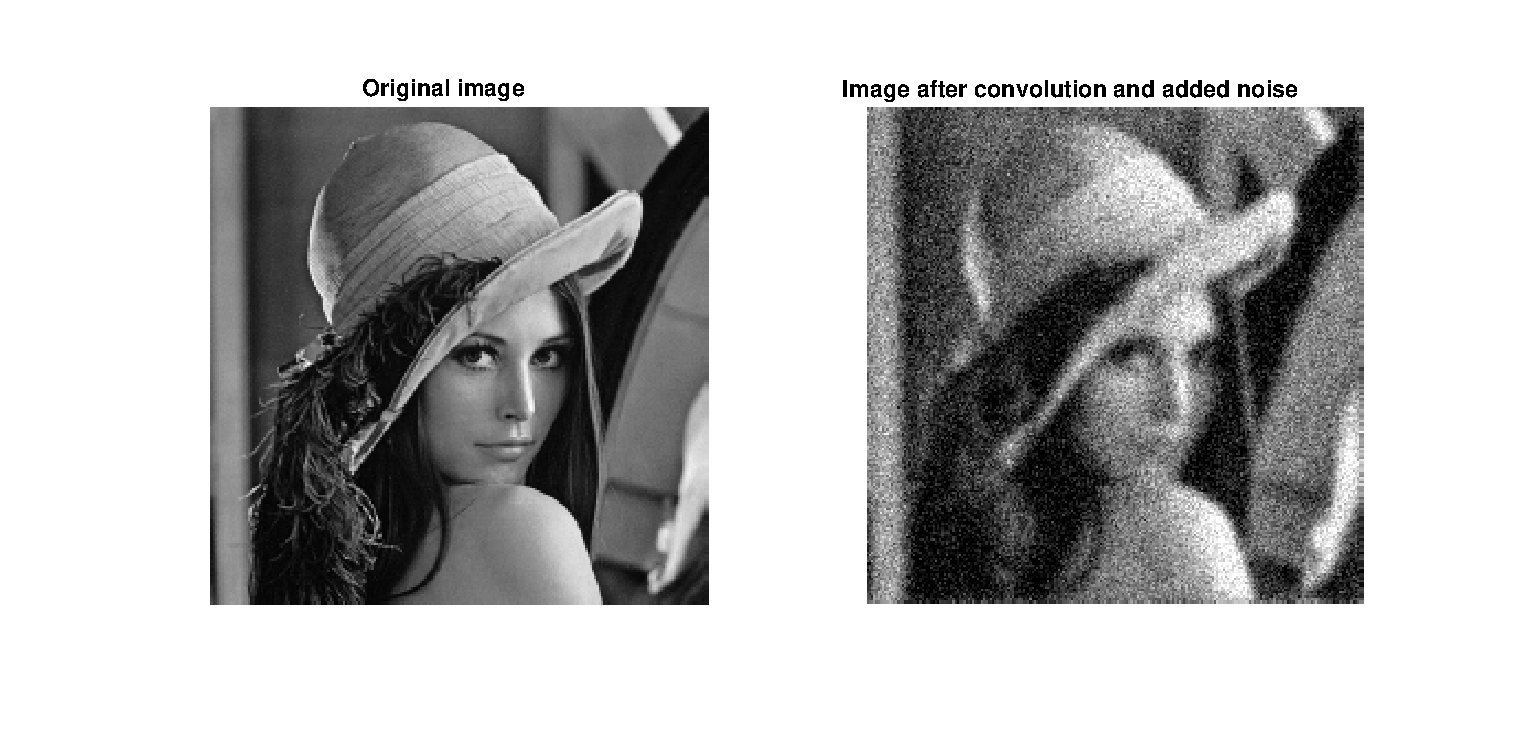
\includegraphics[width=\textwidth]{q4_1.eps}
\caption{Figure showing the original image and the resulting image from convoluting the image \texttt{lena.tif} with a gaussian kernel and then adding gaussian noise.}
  \label{q4_1}
\end{figure}
The linear shift invariantly degraded image is clearly noisy, but the convolution step is harder to see, which is why the window size and standard deviation was changed to make it more noticeable.



\end{document}
